\section{The \pktlanguage compiler}
\label{s:compiler}

% Anirudh->Alvin: This is important I think given the systems context.
% To say how easy it it to build this compiler (in retrospect).
% TODO: Add high-level diagram describing the compiler.
% for every pass, describe what it is, provide an example, show how it's much
% simpler than usual, and show what invariant it guarantees and how it fits
% with the rest of the compiler (Chang had this feedback earlier as well).

We now describe the \pktlanguage compiler. We borrow several well-established
techniques from the compiler literature~\cite{muchnik}. However, as we show
throughout this section, constraining \pktlanguage allows us to considerably
simplify the \pktlanguage compiler relative to mainstream compilers.

\subsection{Lexing, parsing, and semantic analysis}
\pktlanguage's syntax is based on C, implying that \pktlanguage programs are C
programs that can be compiled by a C compiler like clang~\cite{clang}. We use
clang's library interface~\cite{libclang} to generate an Abstract Syntax Tree
(AST) for a packet transaction written in \pktlanguage. The remaining compiler
passes all operate on an AST produced by clang.

Basing \pktlanguage's syntax on C has several benefits. It allows to reuse
clang's industrial strength frontend and catches several compiler programmer
errors with no additional effort. It also allows us to use C's macro
preprocessor for constants. Finally, opaque functions representing hardware
primitives (e.g.  hashes and checksum), can be implemented using arbitrary C
code and linked with \pktlanguage code before running the resulting binary on
our abstract machine.

\subsection{Converting to straight-line code}
A packet transaction's body can contain if-else statements that alter the
program's control flow and complicate dependence analysis. We eliminate if-else
statements by transforming them into the C conditional operator, starting from
the innermost if statements and recursing outwards
(Figure~\ref{fig:if_convert}). This is similar to if
conversion~\cite{allen_if_conversion}, but much simpler because only the if and
else constructs alter control flow in \pktlanguage and all other forms of
control transfers (break, continue, loops) are forbidden.
\begin{figure}[!h]
  \begin{minipage}{0.47\columnwidth}
  \begin{small}
  \begin{lstlisting}[style=customc]
if (pkt.arrival -
    last_time[pkt.id] >
    THRESHOLD) {
 saved_hop[pkt.id] = pkt.new_hop;
}
  \end{lstlisting}
  \end{small}
  \end{minipage}
  \begin{minipage}{0.53\columnwidth}
  \begin{small}
  \begin{lstlisting}[style=customc]
pkt.tmp = pkt.arrival -
          last_time[pkt.id]
          > THRESHOLD;
saved_hop[pkt.id] = pkt.tmp ?
                    pkt.new_hop :
                    saved_hop[pkt.id];
  \end{lstlisting}
  \end{small}
  \end{minipage}
\caption{Conversion to straight-line code}
\label{fig:if_convert}
\end{figure}

This transformation creates straight-line code, where control always passes
from one statement to the next without any branching. Straight-line code
considerably simplifies the rest of the compiler.

\subsection{Identifying state variables}

We next identify all state variables used in a packet transaction, both arrays
and scalars, such as \texttt{last\_time} and \texttt{saved\_hop} in
Figure~\ref{fig:flowlet}. To identify state variables, we scan the
straight-line AST produced by the previous pass, looking for scalar variables
or arrays. For each state variable, we create a \textit{read flank} to read the
state variable into a temporarily created packet field. For an array, we also
move the index expression into the read flank. Here, we use the fact that only
one array address is accessed by each packet in all valid \pktlanguage
programs.  We then replace all occurences of the state variable with the
packet temporary, and create a \textit{write flank} that writes the packet
temporary back into the state variable.  Figure ~\ref{fig:stateful_flanks}
illustrates this transformation on a fragment.

\begin{figure}[!h]
  \begin{minipage}{0.47\columnwidth}
  \begin{small}
  \begin{lstlisting}[style=customc]
pkt.id = hash2(pkt.sport,
               pkt.dport)
         % NUM_FLOWLETS;
last_time[pkt.id] = pkt.arrival;
  \end{lstlisting}
  \end{small}
  \end{minipage}
  \begin{minipage}{0.53\columnwidth}
  \begin{small}
  \begin{lstlisting}[style=customc]
// Read flank for last_time
pkt.id = hash2(pkt.sport,
                pkt.dport)
         % NUM_FLOWLETS;
pkt.last_time = last_time[pkt.id];

pkt.last_time = pkt.arrival;

// Write flank for last_time
last_time[pkt.id] = pkt.last_time;
  \end{lstlisting}
  \end{small}
  \end{minipage}
  \caption{Adding read and write flanks}
\label{fig:stateful_flanks}
\end{figure}

Afer this pass, the code resembles assembly code for a load-store architecture:
state variables are only accessed through reads and writes, and all arithemtic
happens on packet variables. Restricting the set of operations on state
variables allows us to simplify reasoning about state variables during code
partitioning (\S\ref{ss:partitioning}).

\subsection{Static Single-Assignment Form}
We next generate code in static single-assignment form
(SSA)~\cite{ferrante_ssa}, a well-known intermediate form used by many
compilers. In SSA, every variable is assigned exactly once. To compute the SSA,
we replace every definition of a packet variable with a new packet variable and
propagate this new packet variable until the next definition of the same
variable. State variables are already in SSA form because after the flanks have been
added, every state variable is read and written exactly once.
While general algorithms to compute SSA are fairly
involved~\cite{postdominator}, \pktlanguage's SSA computation is much simpler
because it operates on straight-line code.

SSA simplifies further analysis. Because every variable is assigned exactly
once, there are no Write-After-Read or Write-After-Write dependencies; only
Read-After-Write dependencies remain. This, in turn, facilitates dependency analysis
during code partitioning (\S\ref{ss:partitioning}).

\begin{figure}[!h]
  \begin{minipage}{0.48\columnwidth}
  \begin{small}
  \begin{lstlisting}[style=customc]
pkt.id = hash2(pkt.sport,
               pkt.dport)
               % NUM_FLOWLETS;
pkt.last_time = last_time[pkt.id];
pkt.last_time = pkt.arrival;
last_time[pkt.id] = pkt.last_time;
  \end{lstlisting}
  \end{small}
  \end{minipage}
  \begin{minipage}{0.52\columnwidth}
  \begin{small}
  \begin{lstlisting}[style=customc]
pkt.id0 = hash2(pkt.sport,
                pkt.dport)
                % NUM_FLOWLETS;
pkt.last_time0 = last_time[pkt.id0];
pkt.last_time1 = pkt.arrival;
last_time[pkt.id0] = pkt.last_time1;
  \end{lstlisting}
  \end{small}
  \end{minipage}
  \caption{SSA transformation}
\label{fig:ssa}
\end{figure}

\subsection{Three-address code}
We next transform into three-address code, where all instructions are either
reads / writes into stateful variables or carry out packet manipulations of the
form: \texttt{pkt.f1 = pkt.f2 op pkt.f3;} where \texttt{op} includes all
arithmetic, logical, and relational operators. We also allow either pkt.f2 or
pkt.f3 to be an opaque function call of multiple packet fields, because we
assume opaque functions are supported in hardware. Three-address code
instructions are similar to P4's action primitives ~\cite{p4spec} and
RMT~\cite{rmt}'s VLIW instruction set.

To generate three-address code, we flatten expressions that are not already
legal three-address code, by introducing enough temporaries. For instance,
\texttt{pkt.f = pkt.f1 + pkt.f2 - pkt.f3;} would be flattened to
\texttt{pkt.tmp = pkt.f2 - pkt.f3;} followed by \texttt{pkt.f = pkt.f1 +
pkt.tmp;}. Three-address code brings \pktlanguage closer to the hardware,
without yet worrying about issues of concurrency, which we address next.

\begin{figure}[!h]
  \begin{lstlisting}[style=customc]
pkt.id00 = hash2(pkt.sport, pkt.dport) % 8000;
pkt.saved_hop00 = saved_hop[pkt.id00];
pkt.id10 = hash2(pkt.sport, pkt.dport) % 8000;
pkt.last_time00 = last_time[pkt.id10];
pkt.new_hop0 = hash3(pkt.sport, pkt.dport, pkt.arrival_time) % 64;
pkt.tmp1 = pkt.arrival_time - pkt.last_time00;
pkt.tmp00 = pkt.tmp1 > 5;
pkt.saved_hop01 = (pkt.tmp00) ? (pkt.new_hop0) : pkt.saved_hop00;
pkt.last_time01 = pkt.arrival_time;
pkt.next_hop0 = (pkt.tmp00) ? (pkt.new_hop0) : pkt.saved_hop00;
saved_hop[pkt.id00] = (pkt.tmp00) ? (pkt.new_hop0) : pkt.saved_hop00;
last_time[pkt.id10] = pkt.arrival_time;
\end{lstlisting}
\caption{Flowlet switching in three-address code}
\label{fig:three_address}
\end{figure}

\subsection{Code partitioning}
\label{ss:partitioning}
At this point, the code is still in sequential form. Code partitioning
turns sequential code into an atom grid that can be run on \absmachine , by
exploiting parallelism within and across pipeline stages.
To partition code, we carry out the following steps:
\begin{CompactEnumerate}
  \item Create a node for each statement (Figure~\ref{fig:three_address}) in
    the packet transaction after expression flattening.
  \item Create a bidrectional edge between N1 and N2 where N1 is a read from a
    state scalar / state array and N2 is a write into the same state scalar /
    state array. This step captures the constraint that state is internal to an
    atom in \absmachine.
  \item Create an edge (N1, N2) for every pair of nodes N1, N2 where N2 reads
    a variable written by N1. This is the only dependency we need to check because
    control dependencies turn into data dependencies when generating straight-line
    code. Further, the use of SSA removes all write-after-read and write-after-write
    dependencies.
  \item Generate strongly connected components (SCCs) of the resulting graph
    (Figure~\ref{fig:deps}) and condense the SCCs to to create a directed
    acyclic graph (DAG) (Figure~\ref{fig:dag}). This step captures the
    constraint that all updates to state variables must reside within the same
    atom because state is local to an atom.
  \item Schedule the resulting DAG using critical path
    scheduling~\cite{crit_path_sched}, creating a new pipeline stage everytime
    one operation needs to follow another (Figure~\ref{fig:pipeline}).
\end{CompactEnumerate}

\begin{figure*}
  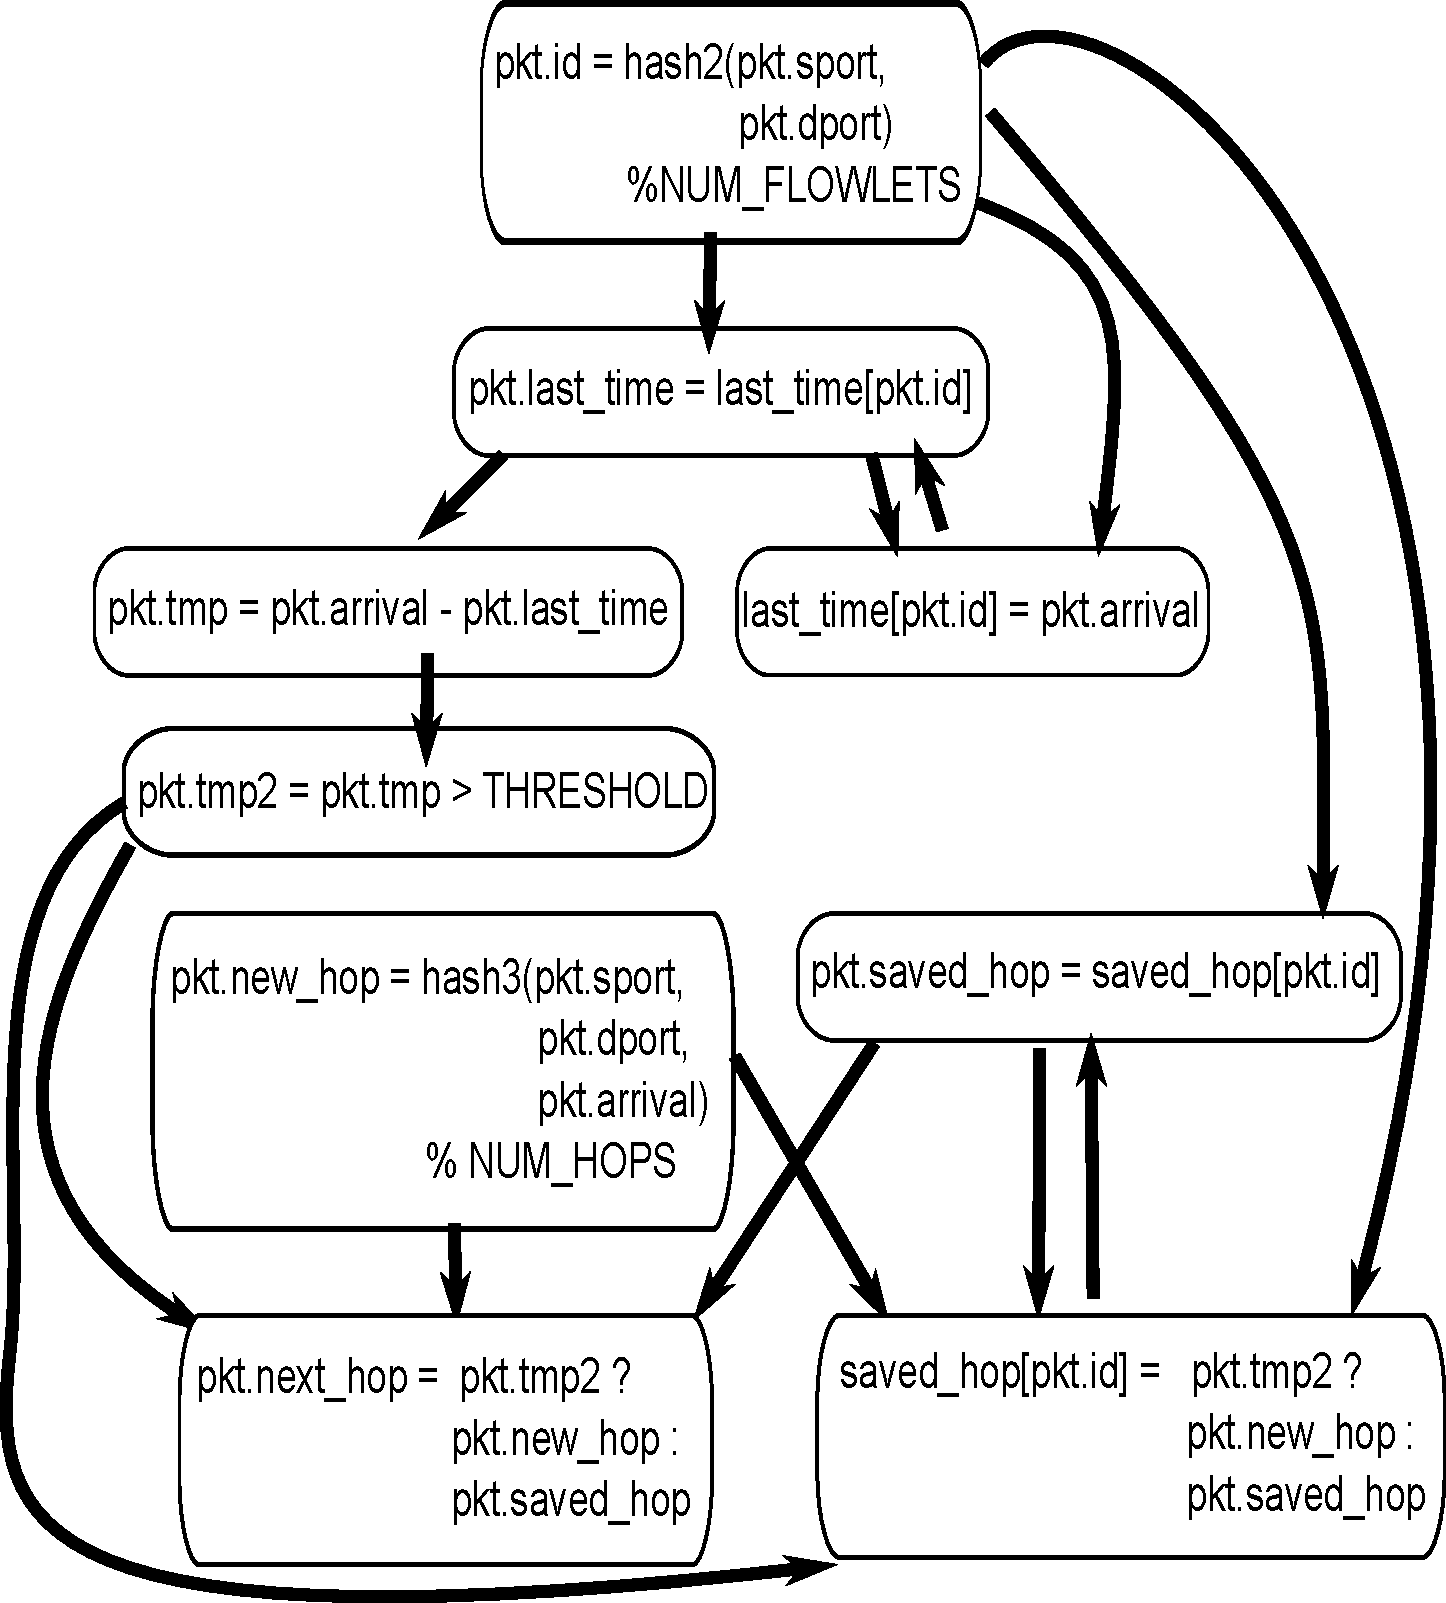
\includegraphics[width=\textwidth]{deps.pdf}
  \caption{Dependency graph of code shown in Figure~\ref{fig:three_address}}
  \label{fig:deps}
\end{figure*}

At this point, each strongly connected component can be turned into an atom for
\absmachine and the resulting pipeline implements the packet transaction.
Further, the atoms have a stylized form. Stateless atoms contain exactly
one three-operand code instruction. Atoms that manipulate state contain at
least two statements: a read from a state variable and a write to a state
variable and optionally consist of one or more updates to the state variable.

\subsection{Constraints on atoms}
\label{ss:complexity}
So far, we haven't constrained the code in atom bodies in any way to reflect
hardware constraints. Expression flattening generates stateless atoms that each
have only one instruction. Further, because these instructions are in
three-operand code form, they map directly to the VLIW capabilities of
programmable switches.

Atoms that manipulate state can, in general, have multi-line atom bodies and it
is unclear whether these can be implemented at all. For instance, the update to
the state variable \texttt{saved\_hop} requires a read, followed by a
conditional update, followed by a write back. We develop a general technique to
determine the implementability of stateful atoms, given constraints on stateful
atom bodies imposed by the hardware.
% Anirudh->Alvin: We seem to be overloading atoms and atom constraints like we
% discussed today afternoon.
We first observe that constraints on stateful atoms can be written as program
sketches~\cite{bitstreaming, finite, sketch_manual}: a code fragment with fixed
and configurable parts. For instance, an atom with the constraint that it can
execute at most one programmable modify operation between a read and a write
operation to a stateful variable x can be represented as:
\begin{figure}
  \begin{lstlisting}[style=customc]
pkt.tmp = x;
pkt.tmp2 = pkt.tmp ?? (??);
x = pkt.tmp;
\end{lstlisting}
\caption{Sketch for single update operation to a state variable}
\label{fig:sketch_for_state}
\end{figure}
Here, the double question mark \texttt{??} stands for a
\textit{hole}~\cite{sketch_manual}. The hole is a placeholder for values from a
finite set that can be substituted in place of the hole. An automated program
synthesis~\cite{synthesis} tool called Sketch~\cite{sketch_manual} then
\textit{fills in} these holes to make the sketch equal to a specification.

As an example, if we want to implement the specification \texttt{x = x + 1;}
using the sketch in Figure~\ref{fig:sketch_for_state}, the Sketch tool would
fill the first hole with the value '+' from the finite set ('+', '-', '/', '*')
and the second hole with the value 1 from a finite set of integers specified as
input to the tool.

For the interested reader, a more detailed explanation of how Sketch works is
available in the appendix. For the purposes of the \pktlanguage compiler
though, we treat Sketch as a blackbox. We express the underlying constraints on
atoms as sketches, feed Sketch with an atom specification that needs to be
satisfied.  If there is a way to complete the sketch to satisfy the atom
specification, Sketch will find it, otherwise, it will determine that the
specification is unsatisfiable. For instance, the specification: \texttt{x = x
* x;} is unsatisfiable given the constraints in
Figure~\ref{fig:sketch_for_state}.

Using sketches to model constraints on atoms allows us to express constraints
very generically and is future proof to changes in hardware capabilities. At
its core, a sketch is an incomplete imperative program, and hence can express a
variety of atom constaints. To show its generality, we conside two such
constraints in our evaluations: an in-order sequential CPU that can execute
exactly $N$ three-operand instructions and a combinatorial circuit with a very
specific form.

\begin{figure}
  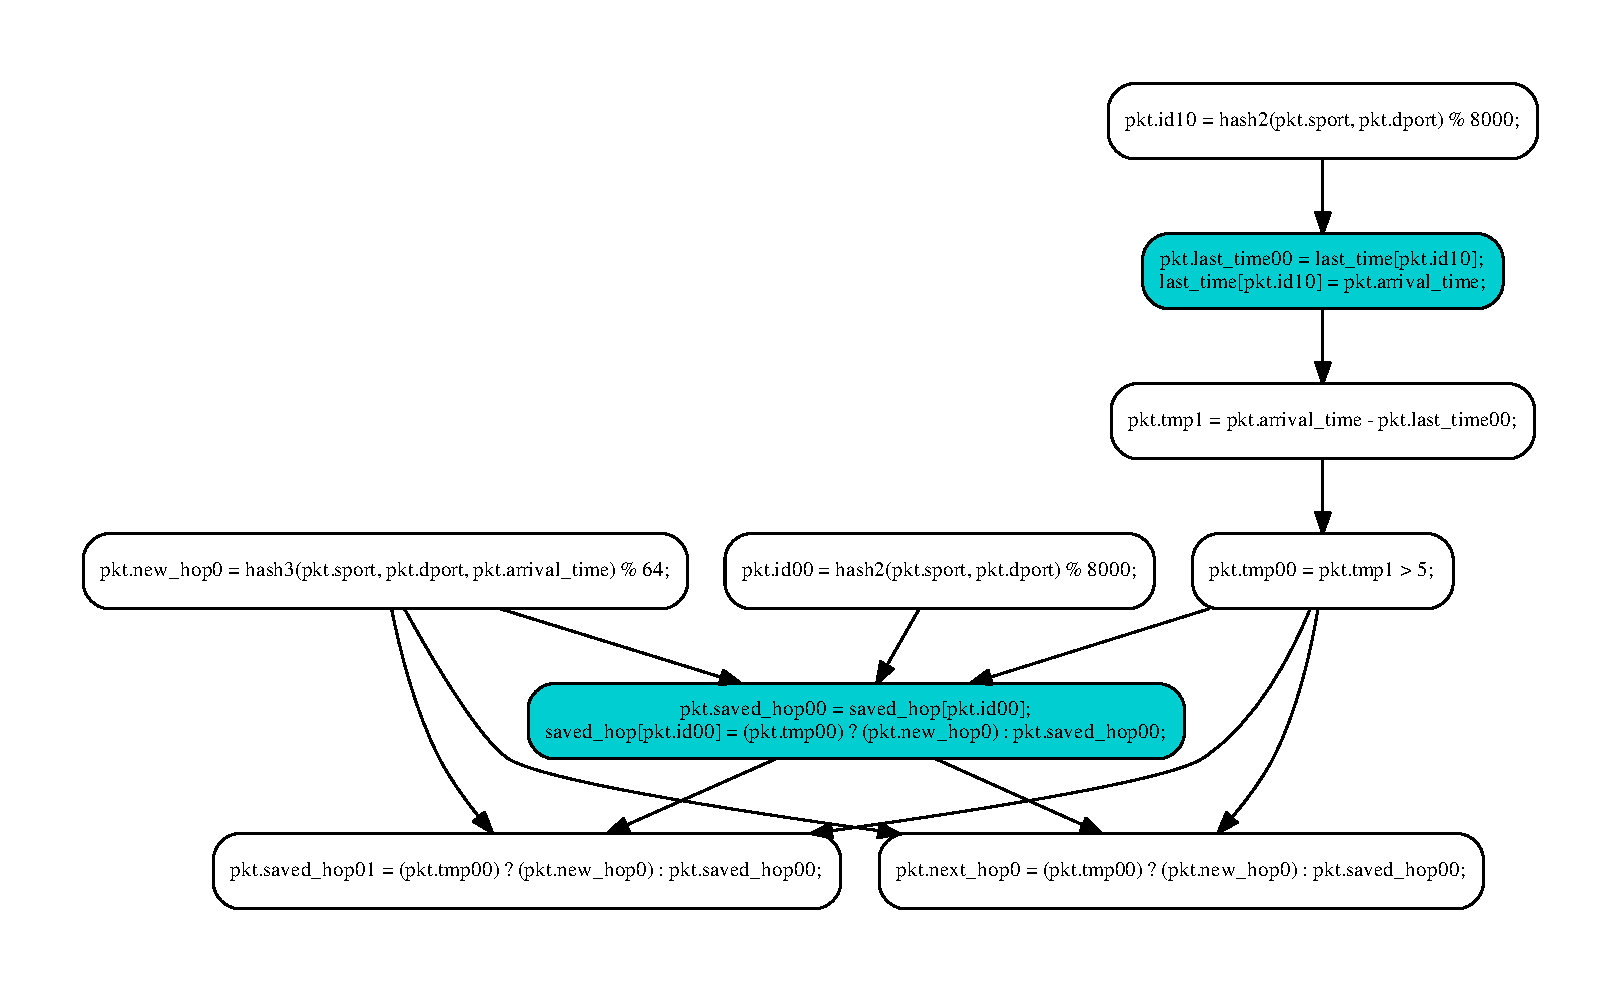
\includegraphics[width=\columnwidth]{dag.pdf}
  \caption{DAG formed by condensing SCCs in Figure~\ref{fig:deps}}
  \label{fig:dag}
\end{figure}

%TODO: Maybe once we have enough examples of optimizations, we can roll those
%into SSA as saying how SSA makes it trivial to apply those optimizations.
% Again, this is compiler 101 for anyone who knows it.

\subsection{Verifying compilations}

To conclude, we describe our testing infrastructure to verify that the
compilation is correct i.e. the externally visible behavior of the packet
transaction (Figure~\ref{fig:flowlet}) is indistinguishable from its pipelined
implementation (Figure~\ref{fig:pipeline}). We verify correctness by feeding in
the same set of test packets to both the packet transaction and its
implementation and comparing the outputs from both programs on the set of
externally visible fields. To create test packets, we scan the packet
transaction and generate the set of all packet fields read from or written to
by the transaction. We then initialize each of these fields by sampling
uniformly from the space of all 32-bit signed integers.

To compare outputs from the packet transaction and its implementation, we track
renames that occur because of SSA. We compare each output field in the
transactional form with the last rename of the same output field in the
implementation. We then feed the same number of test packets to both the
specification and implementation and compare outputs at the end of the
pipeline. This allows to quickly ``spot check'' our compilations and was
instrumental in uncovering a few bugs in various compilation passes during
development.
